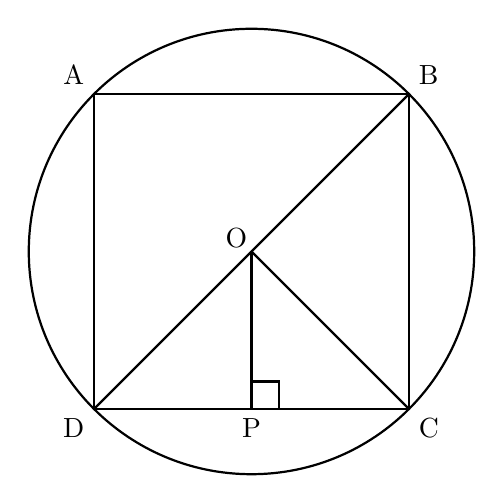
\begin{tikzpicture}[scale=1]

    % Define the coordinates for the center and the vertices of the square
    \coordinate (O) at (0, 0);
    \coordinate (A) at (-2, 2);
    \coordinate (B) at (2, 2);
    \coordinate (C) at (2, -2);
    \coordinate (D) at (-2, -2);
    
    % Define coordinate for point P on segment DC
    \coordinate (P) at (0, -2);

    % Draw the circumscribed circle
    % Radius is the distance from O(0,0) to any vertex, e.g., sqrt(2^2 + 2^2) = sqrt(8) = 2.828
    \draw[thick] (O) circle ({2*sqrt(2)});

    % Draw the square ABCD inscribed in the circle
    \draw[thick] (A) -- (B) -- (C) -- (D) -- cycle;

    % Draw the diagonal connecting D and B
    \draw[thick] (D) -- (B);

    % Draw the line segment from the center O to vertex C
    \draw[thick] (O) -- (C);

    % Draw the line segment from the center O to the midpoint P on DC
    \draw[thick] (O) -- (P);

    % Draw the right-angle indicator at point P
    % It marks the 90-degree angle between OP and PC
    \draw[thick] (0, -1.65) -- (0.35, -1.65) -- (0.35, -2);

    % Add text labels exactly as they appear in the image
    \node[above left] at (A) {A};
    \node[above right] at (B) {B};
    \node[below right] at (C) {C};
    \node[below left] at (D) {D};
    
    % Label O is placed slightly above and to the left of the center
    \node[above left, xshift=2pt, yshift=-2pt] at (O) {O};
    
    % Label P is placed below point P
    \node[below] at (P) {P};

\end{tikzpicture}